\chapter{Arhitektura i dizajn sustava}
		
		Na arhitekturu sustava najveći utjecaj imali su principi oblikovanja: Podijeli pa vladaj, Zadrži razinu apstrakcije te Oblikuj za prenosivost. Princip Podijeli pa vladaj očituje se u podijeli sustava na manje komponente radi povećane razumljivosti te lakše zamjene dijelova i ponovnog korištenja. Princip Zadrži razinu apstrakcije omogućava razumijevanje poante podsustava bez poznavanja nepotrebnih detalja. Korištenje Jave kao objektno orijentiranog programskog jezika omogućuje nam upotrebu razreda, podatkovnih apstrakcija koje sadrže proceduralne apstrakcije (metode). Osim upotrebe razreda Java omogućuje rad na više platformi, čime je osigurana prenosivost.
		
	Organizacija sustava s najviše razine apstrakcije je klijent-poslužitelj-baza podataka. Klijenta predstavlja preglednik weba koji omogućuje korisniku slanje zahtjeva poslužitelju protokolom HTTP \textit{(engl. Hyper Text Transfer Protocol)}. Poslužitelj je server koji poslužuje te zahtjeve, prosljeđuje ih web aplikaciji koja se pokreće preko poslužitelja te vraća odgovore koji se prikazuju preko klijenta (preglednika). Podaci su spremljeni u bazi podataka te joj po potrebi pristupa web aplikacija koristeći SQL upite.
					\begin{figure}[H]
						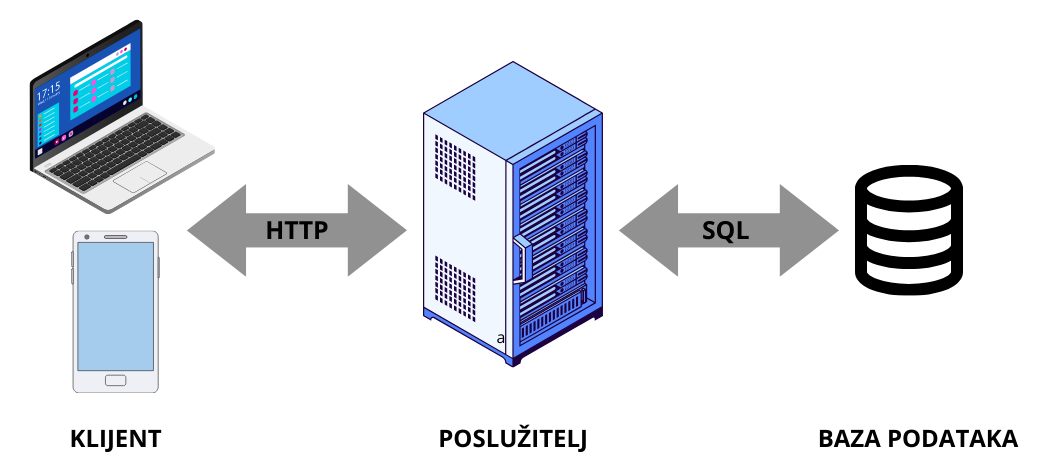
\includegraphics[scale=0.4]{slike/arh1.PNG} %veličina slike u odnosu na originalnu datoteku i pozicija slike
						\centering
						\caption{Organizacija sustava s najviše razine apstrakcije}
						\label{fig:promjene4}
					\end{figure}	
	Arhitektura aplikacije je troslojna. Prvi sloj je \textbf {kontroler} koji prima zahtjeve, poziva odgovarajuće metode drugog sloja \textbf {servisa}, te na kraju vraća odgovore. Servis sadrži poslovnu logiku aplikacije, a za pristup podacima koristi treći sloj \textbf {repozitorij} koji komunicira s bazom podataka.
					\begin{figure}[H]
						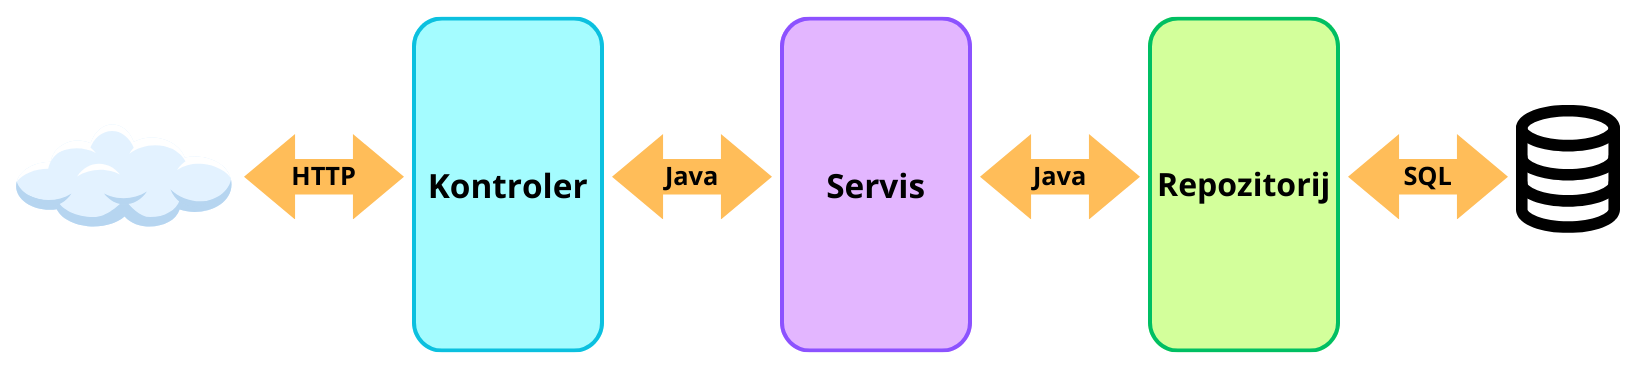
\includegraphics[scale=0.3]{slike/arh2.PNG} %veličina slike u odnosu na originalnu datoteku i pozicija slike
						\centering
						\caption{Organizacija aplikacije}
						\label{fig:promjene5}
					\end{figure}	
	Za izradu naše aplikacije korišten je Java Spring Boot okvir koji koristi MVC \textit{(engl. Model-View-Controller)} oblikovni obrazac u kojem je poslužitelj organiziran u tri dijela u cilju razdvajanja nadležnosti. \textbf {Kontroler} prima zahtjeve koje prosljeđuje modelu te upravlja modelom i pogledom. \textbf {Model} je zadužen za obradu i dohvat podataka te komunicira s bazom podataka. \textbf {Pogled} prezentira dostavljene podatke.
	
		

		

				
		\section{Baza podataka}
		U aplikaciji će baza podataka bit prikazana relacijskim modelom podataka. Objekti relacijskog modela su relacije, a svaka ima jedinstveno ime unutar sheme baze podataka. Relacija je tablica čiji se imenovani stupci nazivaju atributi, a redci n-torke. Ključ entiteta je skup atributa koji jednoznačno određuje entitet. U našem sustavu entiteti baze podataka su:
	\begin{itemize}
		\item Rad
		\item Osoba
		\item Konferencija
		\item Prisutan\_na
		\item Mjesto
		\item Fotografija
		\item Pokrovitelj	
		\item Pokrovitelj\_na
		\item Password\_token	
	\end{itemize}
			\subsection{Opis tablica}
			Entitet \textbf {Rad} sadrži sve važne informacije o radu. Sadrži atribute: ID rada, naziv postera, naziv prezentacije, naslov rada, ID autora, ID konferencije na koju je prijavljen, osvojeni plasman, url postera i prezentacije i ukupan broj osvojenih glasova na toj konferenciji. Atributi naziv prezentacije, url prezentacije i plasman su opcionalni te stoga mogu poprimiti vrijednost null. Entitet Rad u binarnoj je vezi \textit{(Many-to-One)} s entitetom Konferencija i u vezi \textit{(Many-to-One)} s entitetom Osoba.
				\begin{longtblr}[
					label=none,
					entry=none
					]{
						width = \textwidth,
						colspec={|X[7,l]|X[6, l]|X[20, l]|}, 
						rowhead = 1,
					} %definicija širine tablice, širine stupaca, poravnanje i broja redaka naslova tablice
					\hline \SetCell[c=3]{c}{\textbf{Rad}}	 \\ \hline[3pt]
					\SetCell{LightGreen}id & SERIAL	&  	jedinstveni identifikator rada 	\\ \hline
					nazivPoster	& VARCHAR &   	naziv postera koji prikazuje rad\\ \hline 
					nazivPptx & VARCHAR &   naziv prezentacije koja prikazuje rad, može biti null\\ \hline 
					naslov & VARCHAR	&    naslov rada\\ \hline 
					ukupnoGlasova & INT &   ukupan broj osvojenih glasova na konferenciji\\ \hline 
					urlPoster	& VARCHAR &   	url postera koji prikazuje rad\\ \hline 
					urlPptx & VARCHAR &   url prezentacije koja prikazuje rad, može biti null\\ \hline 
					plasman & INT &   plasman na konferenciji, može biti null\\ \hline 
					\SetCell{LightBlue}idKonf	& SERIAL &   	jedinstveni identifikator konferencije\\ \hline 
					\SetCell{LightBlue}idAutor & SERIAL&    jedinstveni identifikator autora\\ \hline 
				\end{longtblr}						
			
			\noindent Entitet \textbf {Osoba} sadrži informacije o autorima, korisnicima te adminima. Sadrži atribute: ID osobe, email, ime i prezime, lozinka (u slučaju da se radi o autoru koji ujedno nije i korisnik bit će null) i uloga koji može poprimiti vrijednosti "admin", "korisnik" ili "autor". Entitet Osoba u binarnoj je vezi s entitetom Rad \textit{(One-to-Many)}, s entitetom Konferencija \textit{(One-to-Many)}, s entitetom Konferencija \textit{(Many-to-Many)} i s entitetom Paassword\_token \textit{(One-to-One)}.
				\begin{longtblr}[
					label=none,
					entry=none
					]{
						width = \textwidth,
						colspec={|X[7,l]|X[6, l]|X[20, l]|}, 
						rowhead = 1,
					} %definicija širine tablice, širine stupaca, poravnanje i broja redaka naslova tablice
					\hline \SetCell[c=3]{c}{\textbf{Osoba}}	 \\ \hline[3pt]
					\SetCell{LightGreen}id & SERIAL	&  	jedinstveni identifikator osobe\\ \hline
					email	& VARCHAR &   	email osobe\\ \hline 
					ime & VARCHAR &   ime osobe\\ \hline 
					prezime & VARCHAR	&    prezime osobe\\ \hline 
					lozinka & VARCHAR &   hash lozinke korisnika ili admina\\ \hline 
					uloga & VARCHAR &  uloga osobe\\ \hline 
				\end{longtblr}		

			\noindent Entitet \textbf {Konferencija} sadrži informacije o stručnoj konferenciji koja će se održati. Sadrži atribute: ID konferencije, poveznica na video prijenos konferencije, pin za ulazak na konferenciju, vrijeme početka i vrijeme kraja konferencije, ID admina zaduženog za konferenciju i adresu i poštanski broj mjesta u kojem se održava konferencija. Entitet Konferencija u binarnoj je vezi s entitetom Rad \textit{(One-to-Many)}, u binarnoj vezi \textit{(Many-to-One)} i \textit{(Many-to-Many)} s entitetom Osoba, u vezi \textit{(Many-to-One)} s entitetom Mjesto, \textit{(One-to-Many)} s entitetom Fotografija i \textit{(Many-to-Many)} s entitetom Pokrovitelj.
				\begin{longtblr}[
					label=none,
					entry=none
					]{
						width = \textwidth,
						colspec={|X[6,l]|X[6, l]|X[20, l]|}, 
						rowhead = 1,
					} %definicija širine tablice, širine stupaca, poravnanje i broja redaka naslova tablice
					\hline \SetCell[c=3]{c}{\textbf{Konferencija}}	 \\ \hline[3pt]
					\SetCell{LightGreen}id & SERIAL	&  	jedinstveni identifikator konferencije \\ \hline
					urlVideo	& VARCHAR &   	 poveznica na direktno video praćenje
trenutnih događanja u glavnoj konferencijskoj dvorani\\ \hline 
					pin & INT &   jedinstveni pin konferencije\\ \hline 
					vrijemePocetak & TIMESTAMP	&    početak konferencije\\ \hline 
					vrijemeKraj & TIMESTAMP	&    kraj konferencije\\ \hline 
					adresa	& VARCHAR &   	 adresa konferencije\\ \hline 
					\SetCell{LightBlue} idAdmin & SERIAL &   jedinstveni identifikator admina zaduženog za konferenciju\\ \hline 
					\SetCell{LightBlue} pbr & INT &   poštanski broj mjesta u kojem se održava konferencija\\ \hline 
				\end{longtblr}		

			\noindent Entitet \textbf {Prisutan\_na} sadrži informacije o prisutnosti pojedinog korisnika na određenoj konferenciji te je li glasao na njoj ili ne. Sadrži atribute: ID konferencije, ID korisnika i glasao. Entitet Prisutan\_na rezultat je binarne veze \textit{(Many-to-Many)} entiteta Osoba s entitetom Konferencija.
				\begin{longtblr}[
					label=none,
					entry=none
					]{
						width = \textwidth,
						colspec={|X[6,l]|X[6, l]|X[20, l]|}, 
						rowhead = 1,
					} %definicija širine tablice, širine stupaca, poravnanje i broja redaka naslova tablice
					\hline \SetCell[c=3]{c}{\textbf{Prisutan\_na}}	 \\ \hline[3pt]
					\SetCell{LightGreen}idKonf & SERIAL	&  	jedinstveni identifikator konferencije \\ \hline
					\SetCell{LightGreen}idKorisnik	& SERIAL &   	jedinstveni identifikator korisnika\\ \hline 
					glasao & BOOLEAN &   informacija je li korisnik već glasao na konferenciji\\ \hline 
				\end{longtblr}

			\noindent Entitet \textbf {Mjesto} sadrži informacije o pojedinom mjestu. Sadrži atribute: poštanski broj i naziv mjesta. Entitet Mjesto u binarnoj je vezi s entitetom Konferencija \textit{(One-to-Many)}. 
				\begin{longtblr}[
					label=none,
					entry=none
					]{
						width = \textwidth,
						colspec={|X[6,l]|X[6, l]|X[20, l]|}, 
						rowhead = 1,
					} %definicija širine tablice, širine stupaca, poravnanje i broja redaka naslova tablice
					\hline \SetCell[c=3]{c}{\textbf{Mjesto}}	 \\ \hline[3pt]
					\SetCell{LightGreen}pbr & INT &   poštanski broj mjesta \\ \hline
					naziv	& VARCHAR &   	naziv mjesta\\ \hline 
				\end{longtblr}

			\noindent Entitet \textbf {Fotografija} sadrži informacije o uslikanoj fotografiji te na kojoj konferenciji je uslikana. Sadrži atribute: ID fotografije, url fotografije i ID konferencije. Entitet Fotografija u binarnoj je vezi s entitetom Konferencija \textit{(Many-to-One)}. 
				\begin{longtblr}[
					label=none,
					entry=none
					]{
						width = \textwidth,
						colspec={|X[6,l]|X[6, l]|X[20, l]|}, 
						rowhead = 1,
					} %definicija širine tablice, širine stupaca, poravnanje i broja redaka naslova tablice
					\hline \SetCell[c=3]{c}{\textbf{Fotografija}}	 \\ \hline[3pt]
					\SetCell{LightGreen}id & SERIAL	&  	jedinstveni identifikator fotografije\\ \hline
					urlSlike	& VARCHAR &   	url fotografije\\ \hline 
					\SetCell{LightBlue}idKonf & SERIAL &   jedinstveni identifikator konferencije\\ \hline 
				\end{longtblr}

			\noindent Entitet \textbf {Pokrovitelj} sadrži informacije o pokrovitelju. Sadrži atribute: ID pokrovitelja,  url stranice pokrovitelja, naziv pokrovitelja i url slike. Entitet Pokrovitelj u binarnoj je vezi s entitetom Konferencija \textit{(Many-to-Many)}. 
				\begin{longtblr}[
					label=none,
					entry=none
					]{
						width = \textwidth,
						colspec={|X[7,l]|X[6, l]|X[20, l]|}, 
						rowhead = 1,
					} %definicija širine tablice, širine stupaca, poravnanje i broja redaka naslova tablice
					\hline \SetCell[c=3]{c}{\textbf{Pokrovitelj}}	 \\ \hline[3pt]
					\SetCell{LightGreen}id & SERIAL	&  	jedinstveni identifikator pokrovitelja\\ \hline
					url	& VARCHAR &   	poveznica na stranicu pokrovitelja\\ \hline 
					naziv	& VARCHAR &   	naziv pokrovitelja\\ \hline 
					urlSlike	& VARCHAR &   	logo pokrovitelja\\ \hline
				\end{longtblr}

			\noindent Entitet \textbf {Pokrovitelj\_na} sadrži informacije o uključenosti pokrovitelja na pojedinoj konferenciji. Sadrži atribute: ID konferencije i ID pokrovitelja. Entitet Pokrovitelj\_na rezultat je binarne veze \textit{(Many-to-Many)} entiteta Pokrovitelj i Konferencija.
				\begin{longtblr}[
					label=none,
					entry=none
					]{
						width = \textwidth,
						colspec={|X[6,l]|X[6, l]|X[20, l]|}, 
						rowhead = 1,
					} %definicija širine tablice, širine stupaca, poravnanje i broja redaka naslova tablice
					\hline \SetCell[c=3]{c}{\textbf{Pokrovitelj\_na}}	 \\ \hline[3pt]
					\SetCell{LightGreen}idKonf & SERIAL	&  	jedinstveni identifikator konferencije \\ \hline
					\SetCell{LightGreen}idPokrovitelj	& SERIAL &   	jedinstveni identifikator pokrovitelja\\ \hline 
				\end{longtblr}
			\noindent Entitet \textbf {Password\_token} sadrži informacije o tokenu koji je pojedina osoba dobila kada je zatražila promjenu lozinke. Sadrži atribute: ID tokena, istek tokena, token i ID osobe čiji je token. Entitet Password\_token u binarnoj je vezi s entitetom Osoba \textit{(One-to-One)}. .
				\begin{longtblr}[
					label=none,
					entry=none
					]{
						width = \textwidth,
						colspec={|X[6,l]|X[6, l]|X[20, l]|}, 
						rowhead = 1,
					} %definicija širine tablice, širine stupaca, poravnanje i broja redaka naslova tablice
					\hline \SetCell[c=3]{c}{\textbf{Pokrovitelj\_na}}	 \\ \hline[3pt]
					\SetCell{LightGreen}id & SERIAL	&  	jedinstveni identifikator tokena \\ \hline
					istek	& DATE &   	datum isteka tokena\\ \hline 
					token	& VARCHAR &   	token\\ \hline 
					\SetCell{LightBlue}idOsoba & SERIAL &   jedinstveni identifikator osobe\\ \hline 
				\end{longtblr}
			\subsection{Dijagram baze podataka}
%				\textit{ U ovom potpoglavlju potrebno je umetnuti dijagram baze podataka. Primarni i strani ključevi moraju biti označeni, a tablice povezane. Bazu podataka je potrebno normalizirati. Podsjetite se kolegija "Baze podataka".}
					\begin{figure}[H]
						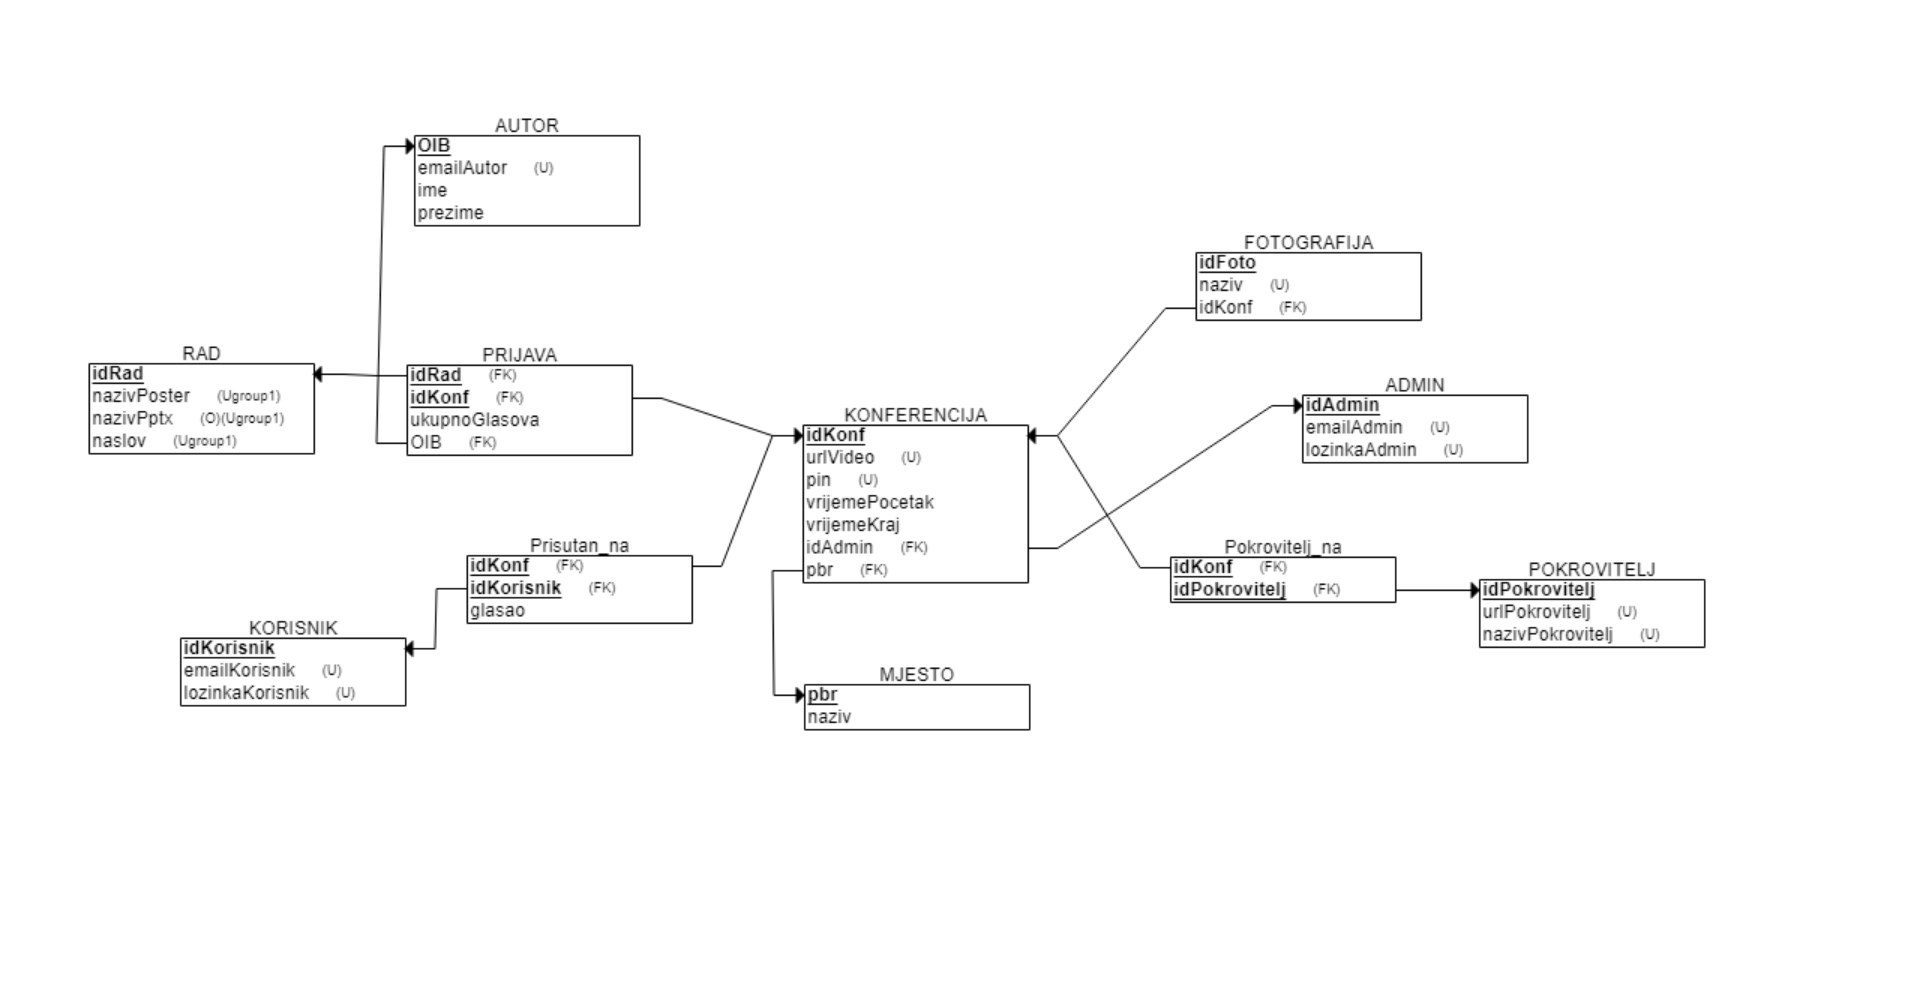
\includegraphics[scale=0.55]{dijagrami/dijagram baze podataka.PNG} %veličina slike u odnosu na originalnu datoteku i pozicija slike
						\centering
						\caption{Dijagram baze podataka}
						\label{fig:promjene3}
					\end{figure}			
			\eject
			
			
		\section{Dijagram razreda}
		
		
			Radi preglednosti, dijagram je razlomljen na nekoliko dijelova. Na njima su prikazani razredi koji pripadaju backend dijelu MVC arhitekture.
			Na slici 4.4 je prikazan Model dio. Model klase služe za prijenos podataka između baze podataka i serverske strane aplikacije. Ti su objekti zapravo preslika baze podataka, ali umjesto relacijske koristimo objektno-orijentiranu paradigmu. 
			Razred Konferencija predstavlja konferenciju koja se prikazuje u aplikaciji. 
Razred Mjesto predstavlja lokaciju na kojoj se konferencija održava.
Razred Osoba predstavlja čovjeka koji na neki način sudjeluje na konferenciji.  Taj razred ima atribut uloga kojim se određuje je li ta osoba autor, administrator ili posjetitelj konferencije. 
Razred Rad predstavlja rad (poster i/ili pptx) kojim se autor predstavlja na konferenciji.
Razred PrisutanNa omogućuje da pratimo tko je na konferenciji te da li je ta osoba glasala za neki rad.
Razred Fotografija predstavlja fotografije konferencije koje administrator stavlja u aplikaciju tijekom ili nakon konferencije.
Razred Pokrovitelj predstavlja sponzore konferencije. 
Razred PasswordToken omogućuje postavljanje i promjenu lozinku.
Razred Media omogućuje lakši prikaz i pohranu medijskih sadržaja.

			\begin{figure}[H]
				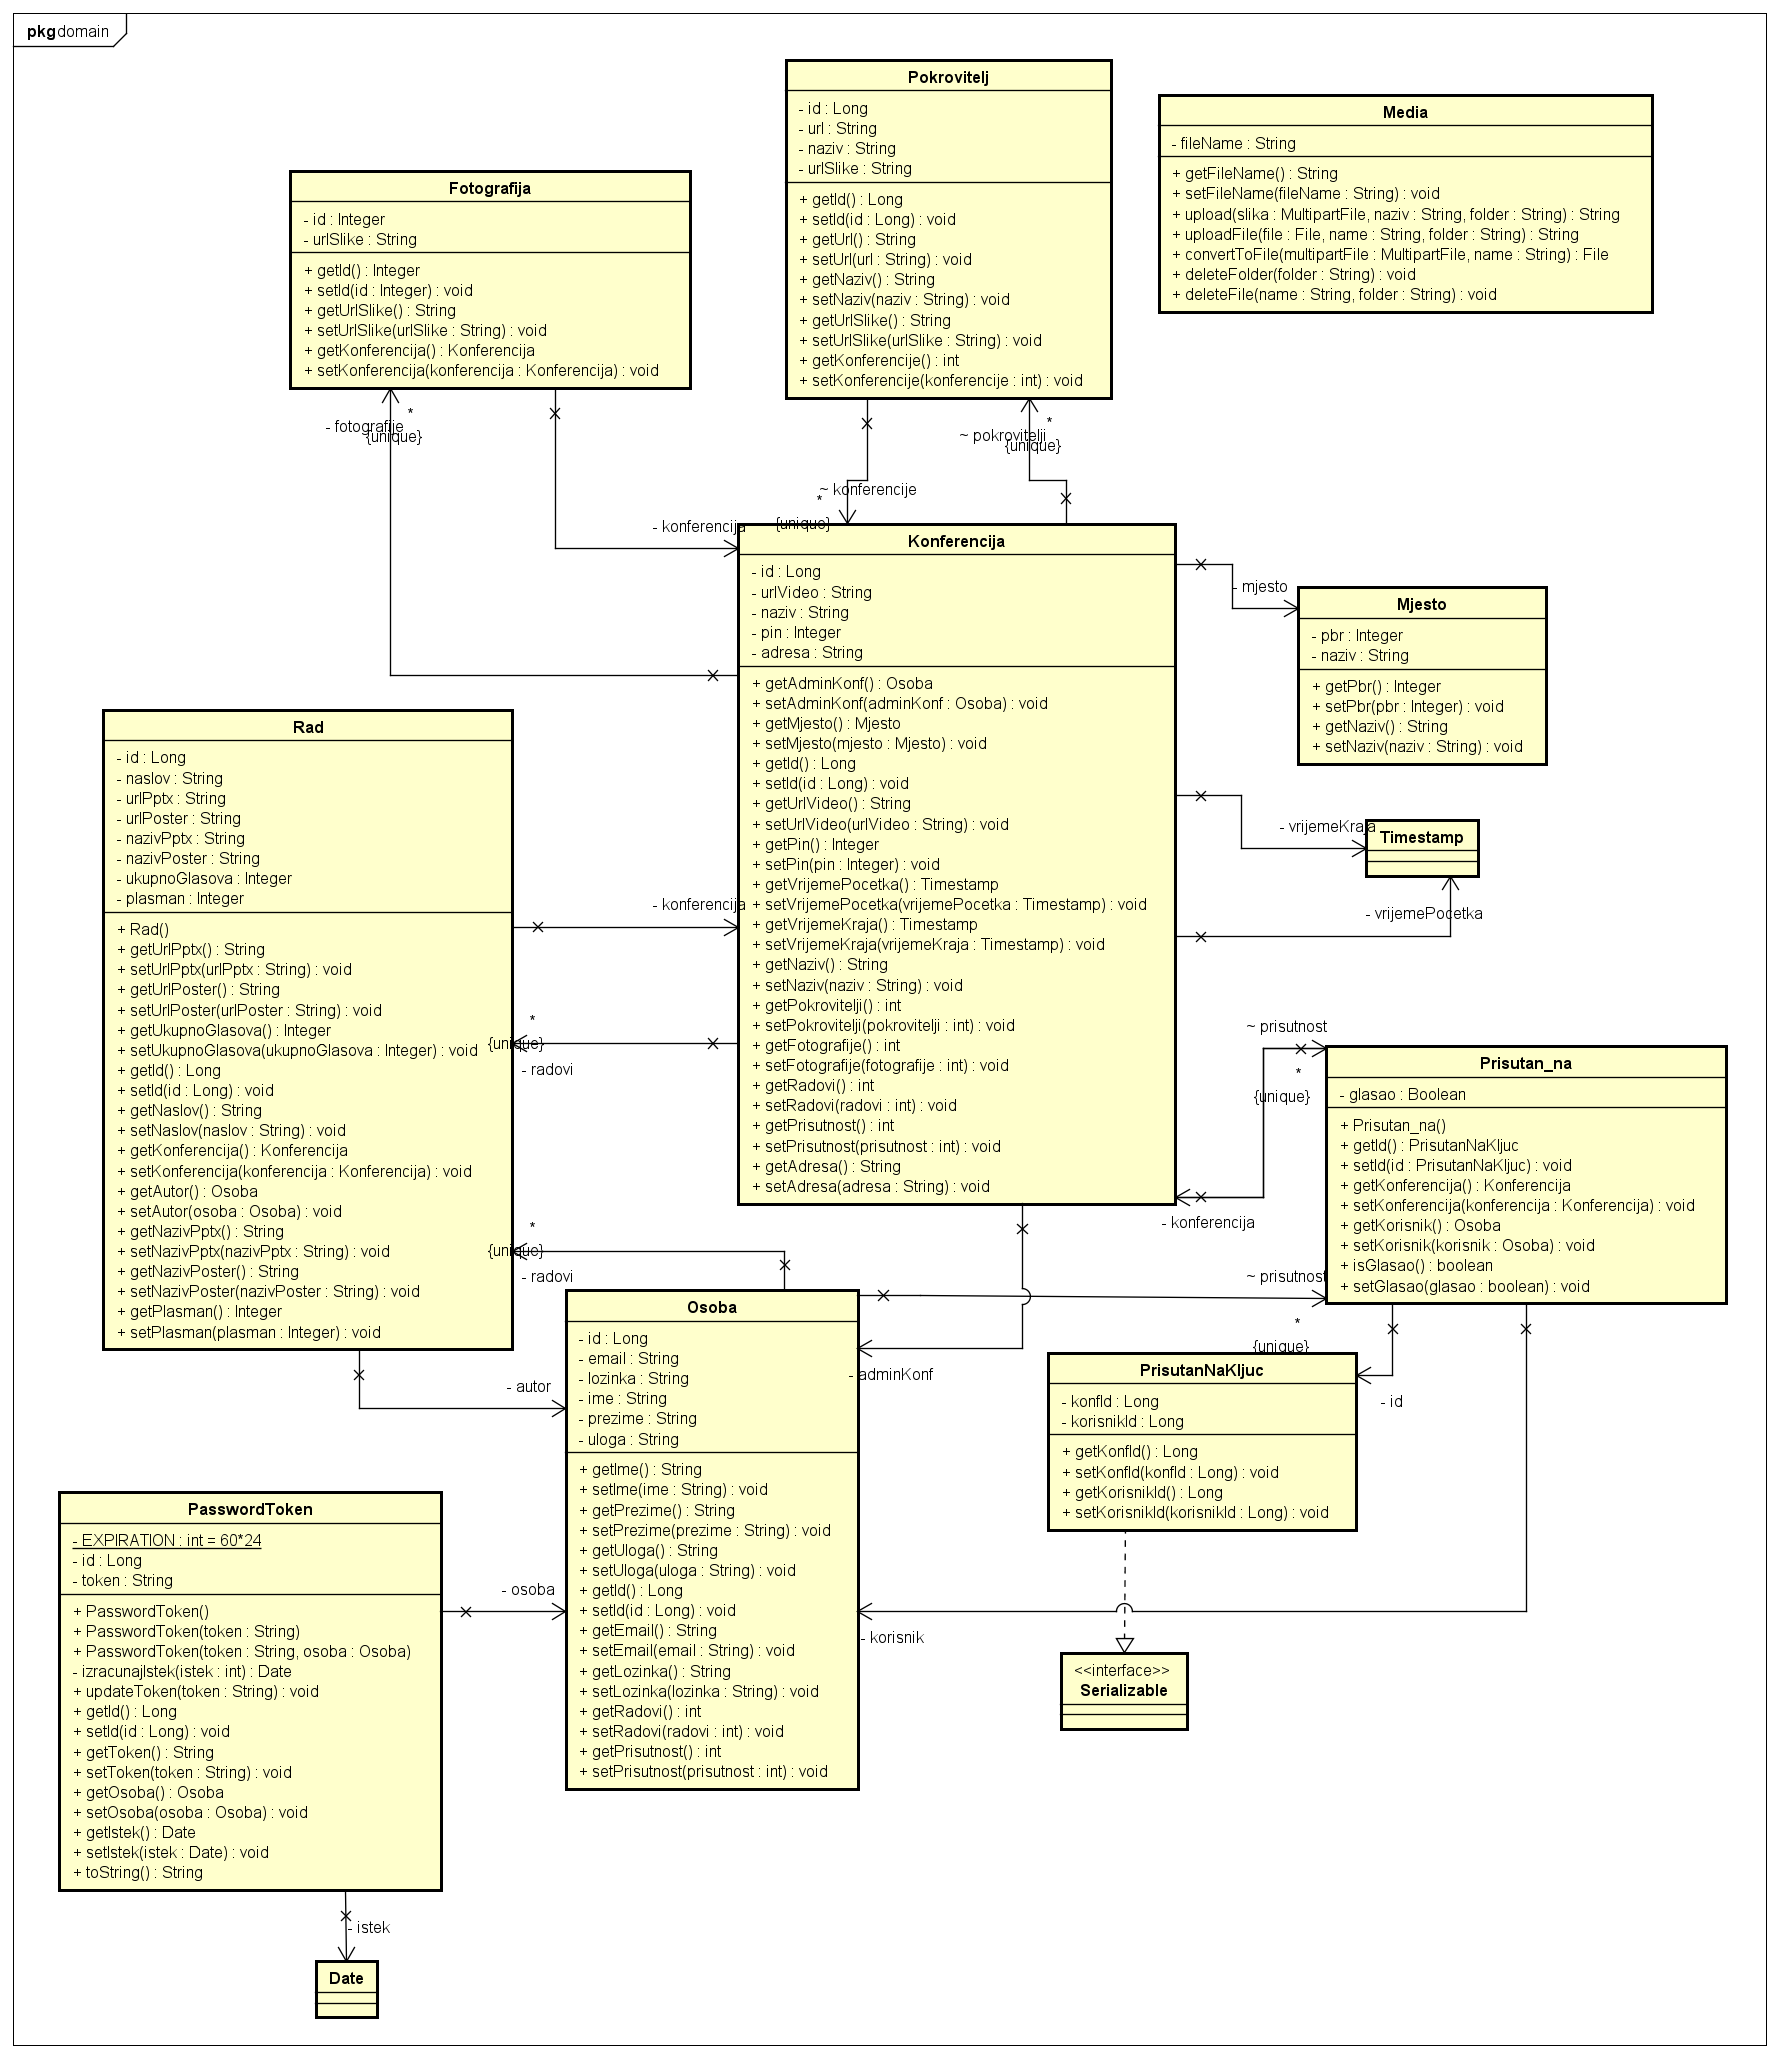
\includegraphics[scale=0.35]{dijagrami/models.png}%veličina slike u odnosu na originalnu datoteku i pozicija slike
				\centering
				\caption{Dijagram razreda - dio Models}
				\label{fig:promjena9}
			\end{figure}
			

			Na slikama 4.5, 4.6 i 4.7 je prikazan glavni dijagram u čijem središtu se nalazi JPARepository o kojem ovise ostala sučelja koja su specifična za svaki objekt. Ova sučelja nam omogućuju da izbjegnemo pisanje složenih SQL upita i umjesto toga koristimo generičke metode za izvođenje uobičajenih operacija s bazom podataka.
U dijagramu su i servisi u kojima su funkcije za obradu podataka. Po potrebi zovu repozitorijeve funkcije kako bi došli do baze podataka.
Kontroleri nam služe za komunikaciju s frontendom. 
U klasi PosterizedApplication se nalazi glavna funkcija za pokretanje aplikacije. WebSecurityBasic je zadužen za zaštitu cijele aplikacije.

			

			\begin{figure}[H]
				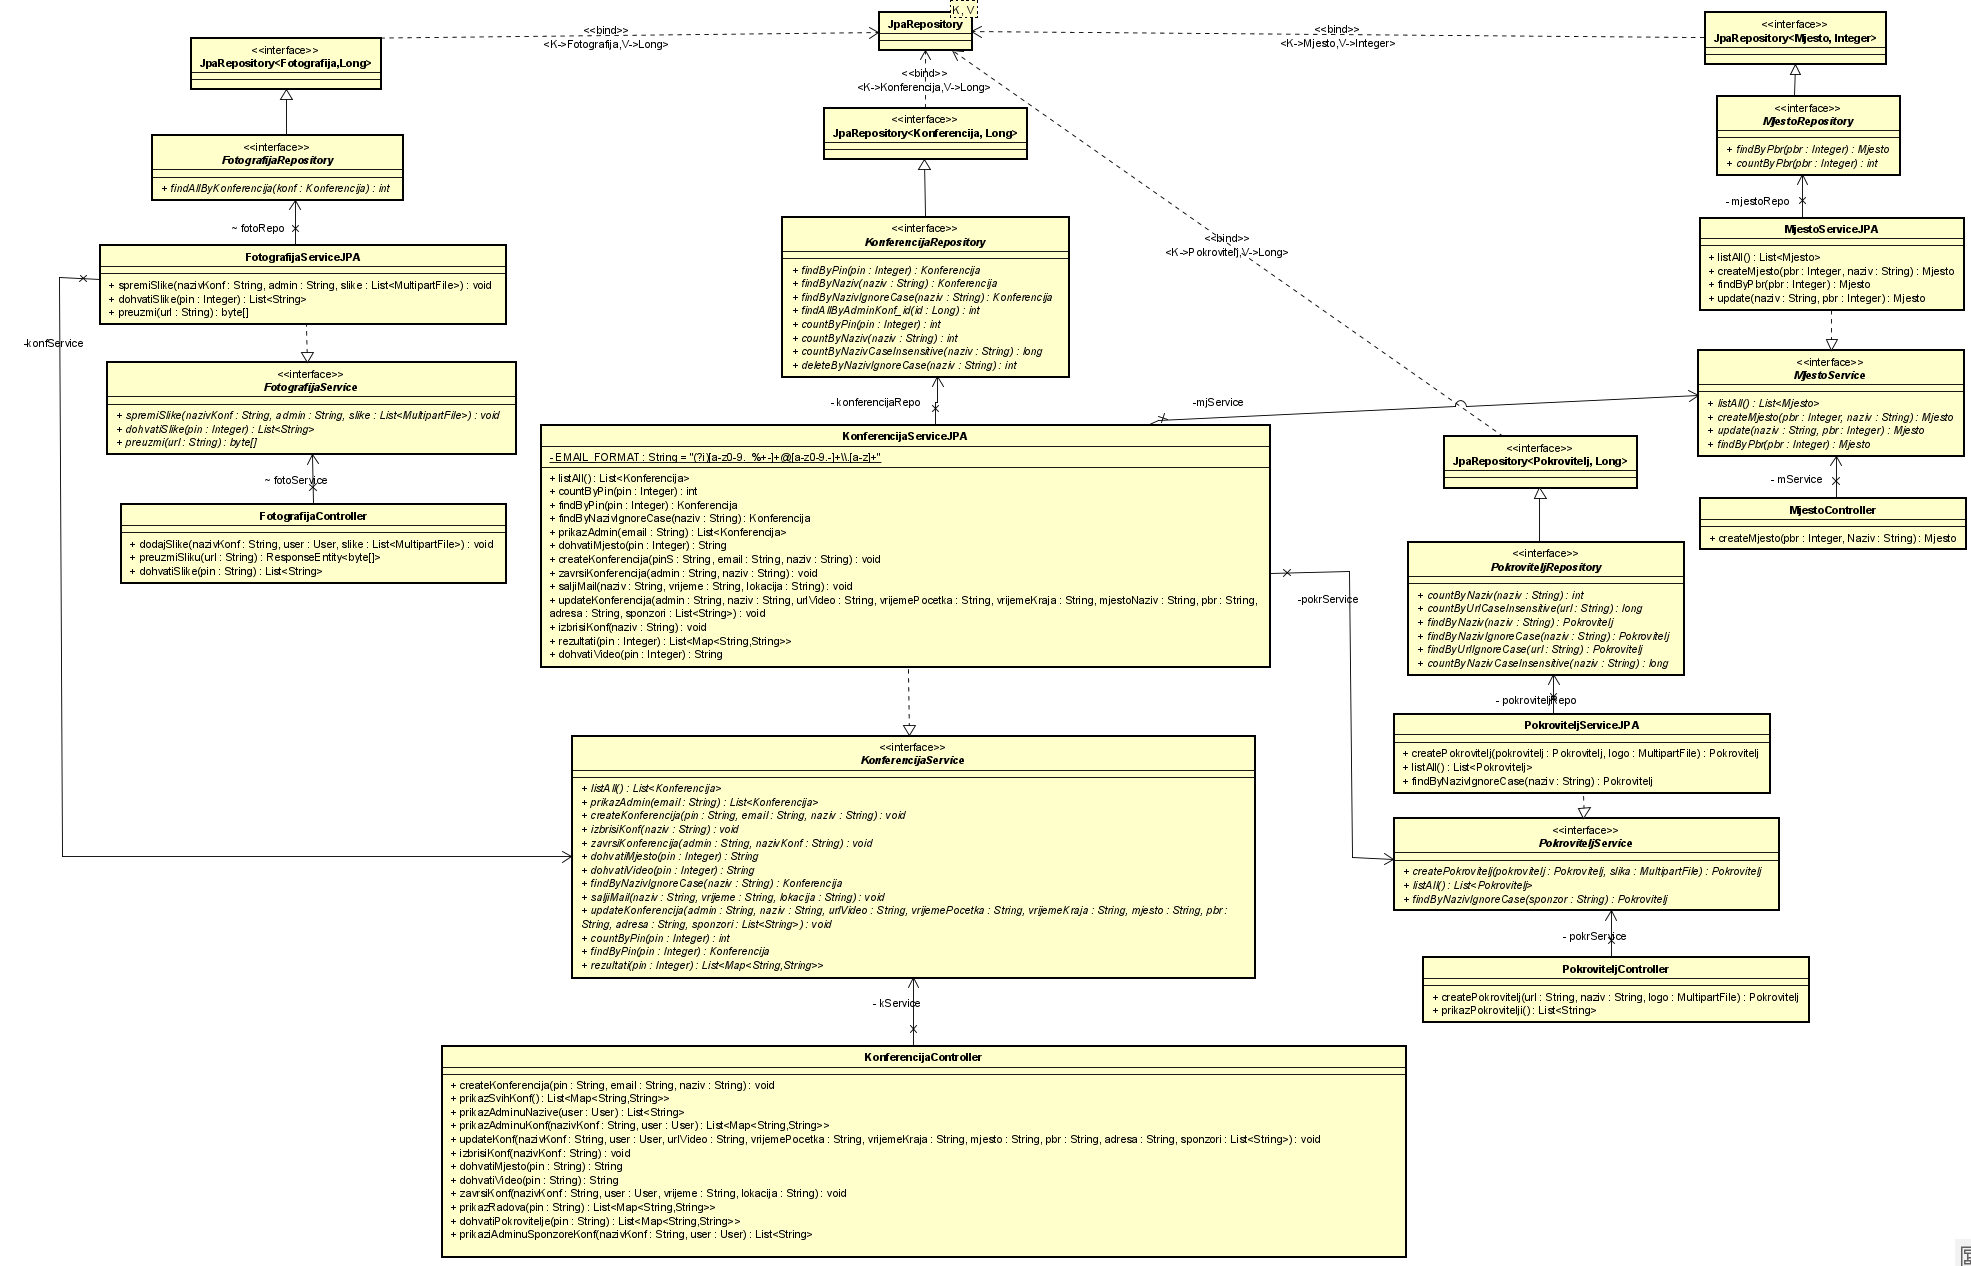
\includegraphics[scale=0.5]{dijagrami/glavni_1.png}%veličina slike u odnosu na originalnu datoteku i pozicija slike
				\centering
				\caption{Dijagram razreda - glavni dijagram 1.dio}
				\label{fig:promjena9.1}
			\end{figure}
			
			\begin{figure}[H]
				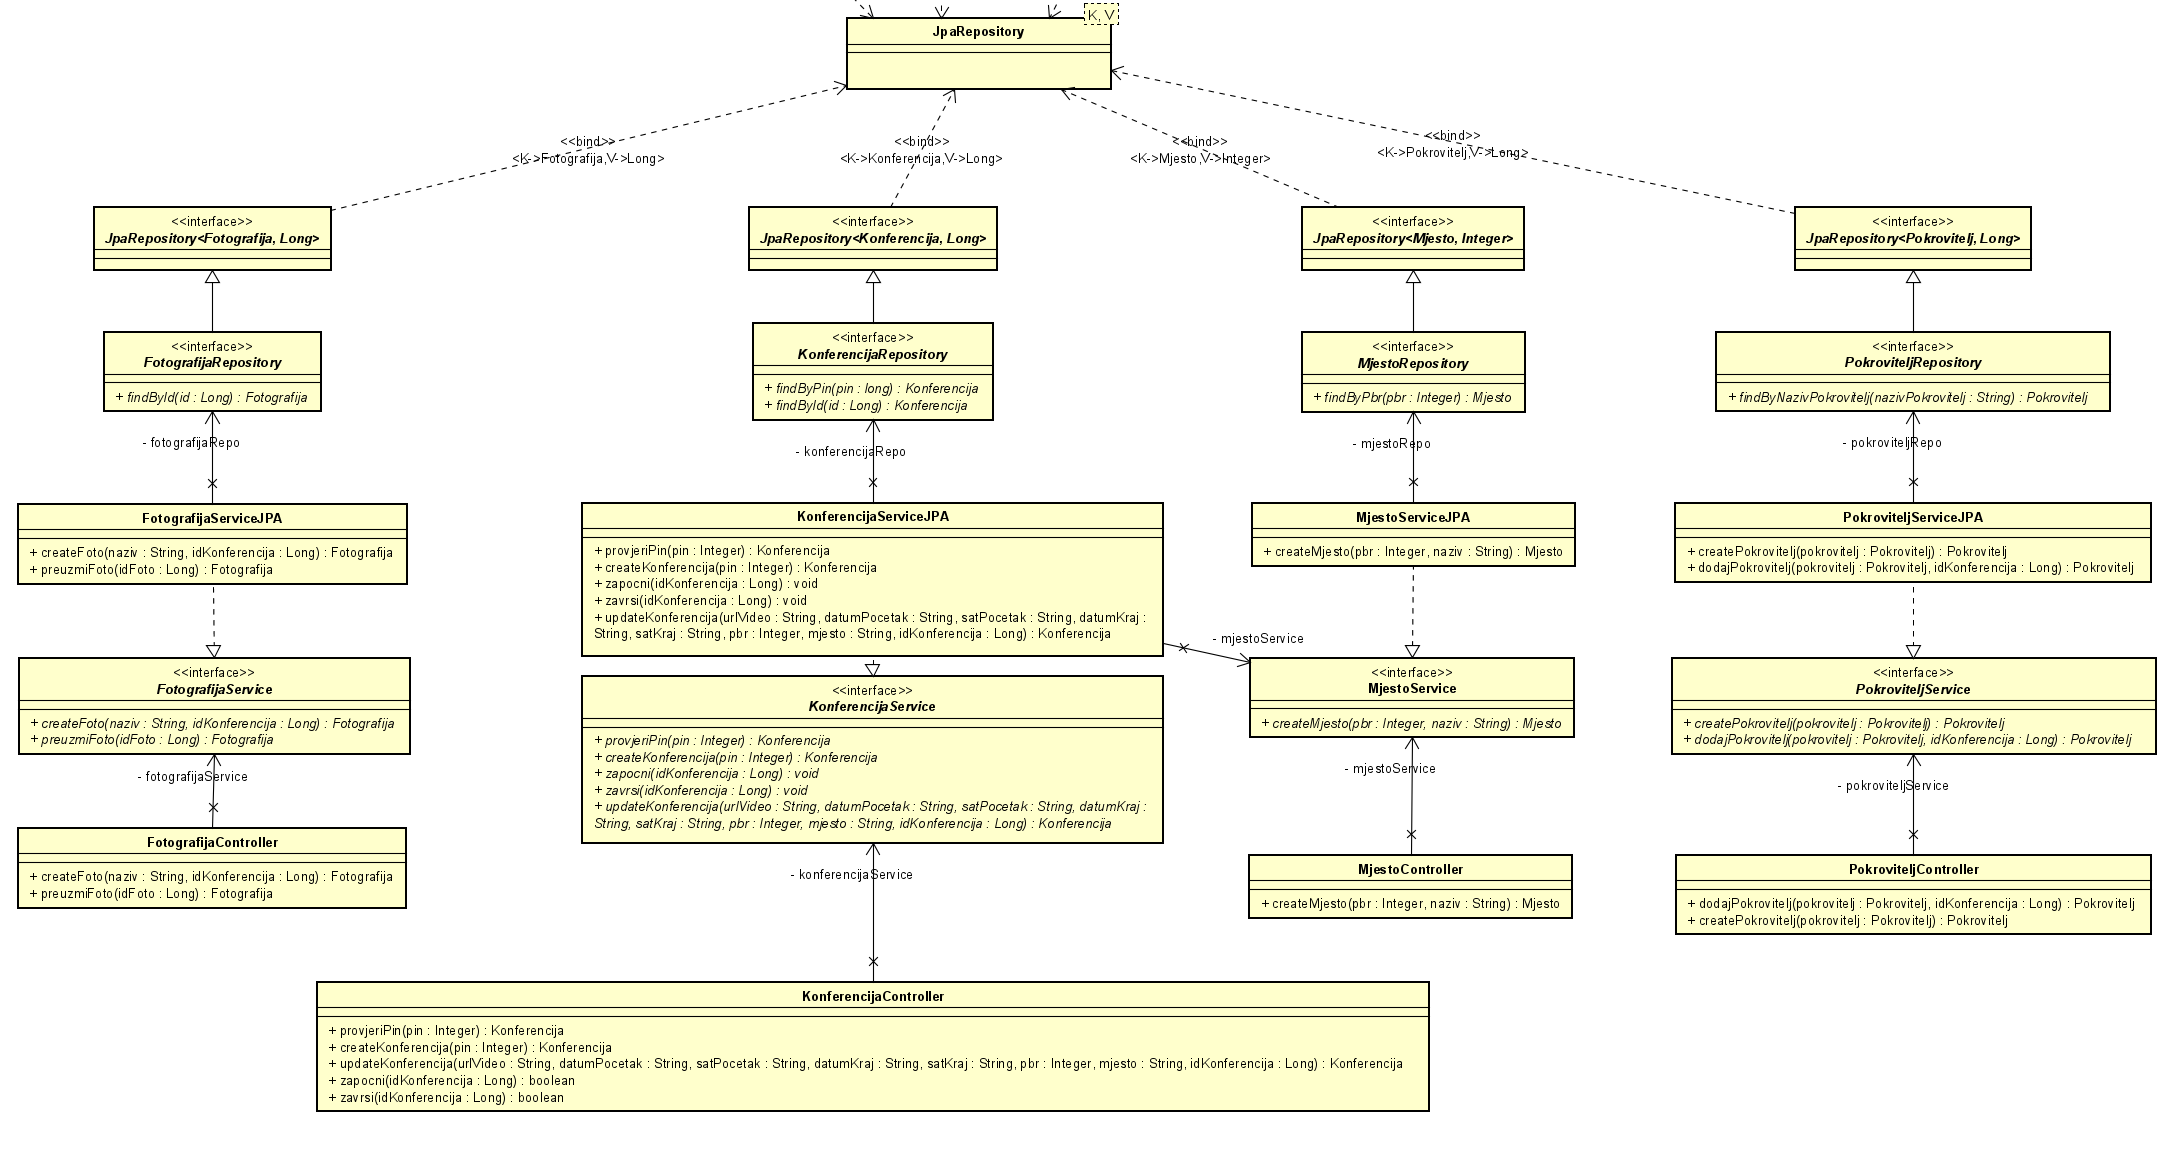
\includegraphics[scale=0.5]{dijagrami/glavni_2.png}%veličina slike u odnosu na originalnu datoteku i pozicija slike
				\centering
				\caption{Dijagram razreda - glavni dijagram 2.dio}
				\label{fig:promjena9.2}
			\end{figure}
			
			\begin{figure}[H]
				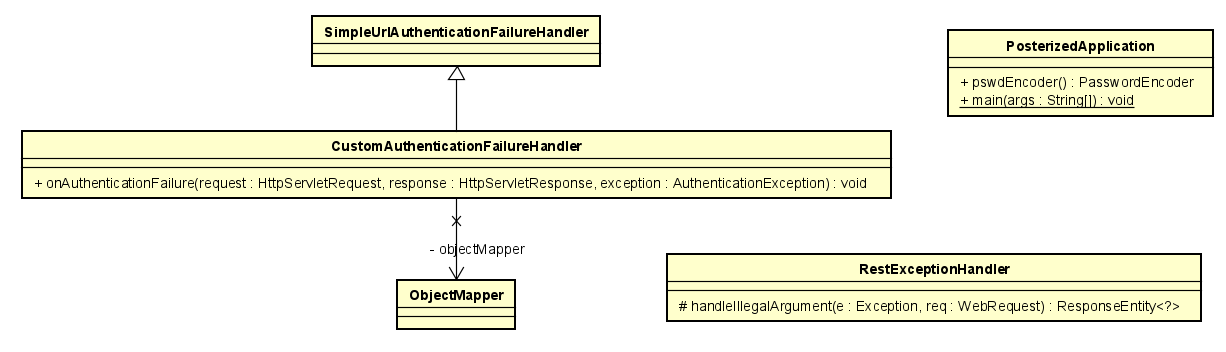
\includegraphics[scale=0.5]{dijagrami/glavni_3.png}%veličina slike u odnosu na originalnu datoteku i pozicija slike
				\centering
				\caption{Dijagram razreda - glavni dijagram 3.dio}
				\label{fig:promjena9.3}
			\end{figure}

			
			
			
			
			
			\eject
		
		\section{Dijagram stanja}

			Dijagram stanja je vrsta dijagrama koji se koristi u inženjerstvu softvera za prikazivanje različitih stanja kroz koja objekt ili interakcija prolazi tijekom svog životnog ciklusa. Obuhvaća stanja, prijelaze i događaje koji uzrokuju promjene iz jednog stanja u drugo. Korisan je u fazi dizajna jer pomaže u razumijevanju i vizualizaciji kako korisnici interagiraju s sustavom, te kako se sustav ponaša u različitim situacijama.
			
			Početno stanje je "Početna stranica", iz koje korisnik može prijeći na "Prijava" ako odabere "Prijava" ili "Prikaži obrazac za prijavu". Ukoliko je prijava neuspješna, korisnik ostaje na početnoj stranici. U slučaju uspješne prijave, korisnik prelazi u stanje "Početna stranica – prijavljen korisnik" što je ustvari proširenje prvobitne početne stranice. 
			
			Daljnje mogućnosti uključuju odabir "Odjava" (korisnika) za povratak na početno stanje, "Livestream" za praćenje video prijenosa konferencije, "Galerija" za pregled galerije fotografija (s različitim ishodima ovisno o tome jesu li fotografije poslane ili ne), "Preuzmi" za pohranjivanje fotografija, te "Glasaj" za pregled radova i glasanje za poster te "Unos pina" za dodavanje konferencije.
			
			Na desnom dijelu dijagrama nalazi se stanje "Prikaži konferenciju", gdje korisnik može pristupiti konferenciji ako je PIN kod ispravan ili ostati na istoj stranici ako PIN kod nije ispravan. U tom stanju dostupne su osnovne informacije o konferenciji, vremenska prognoza te pokrovitelji.
			
			Dijagram je prikazan na sljedećoj stranici.

			
			\begin{figure}[H]
				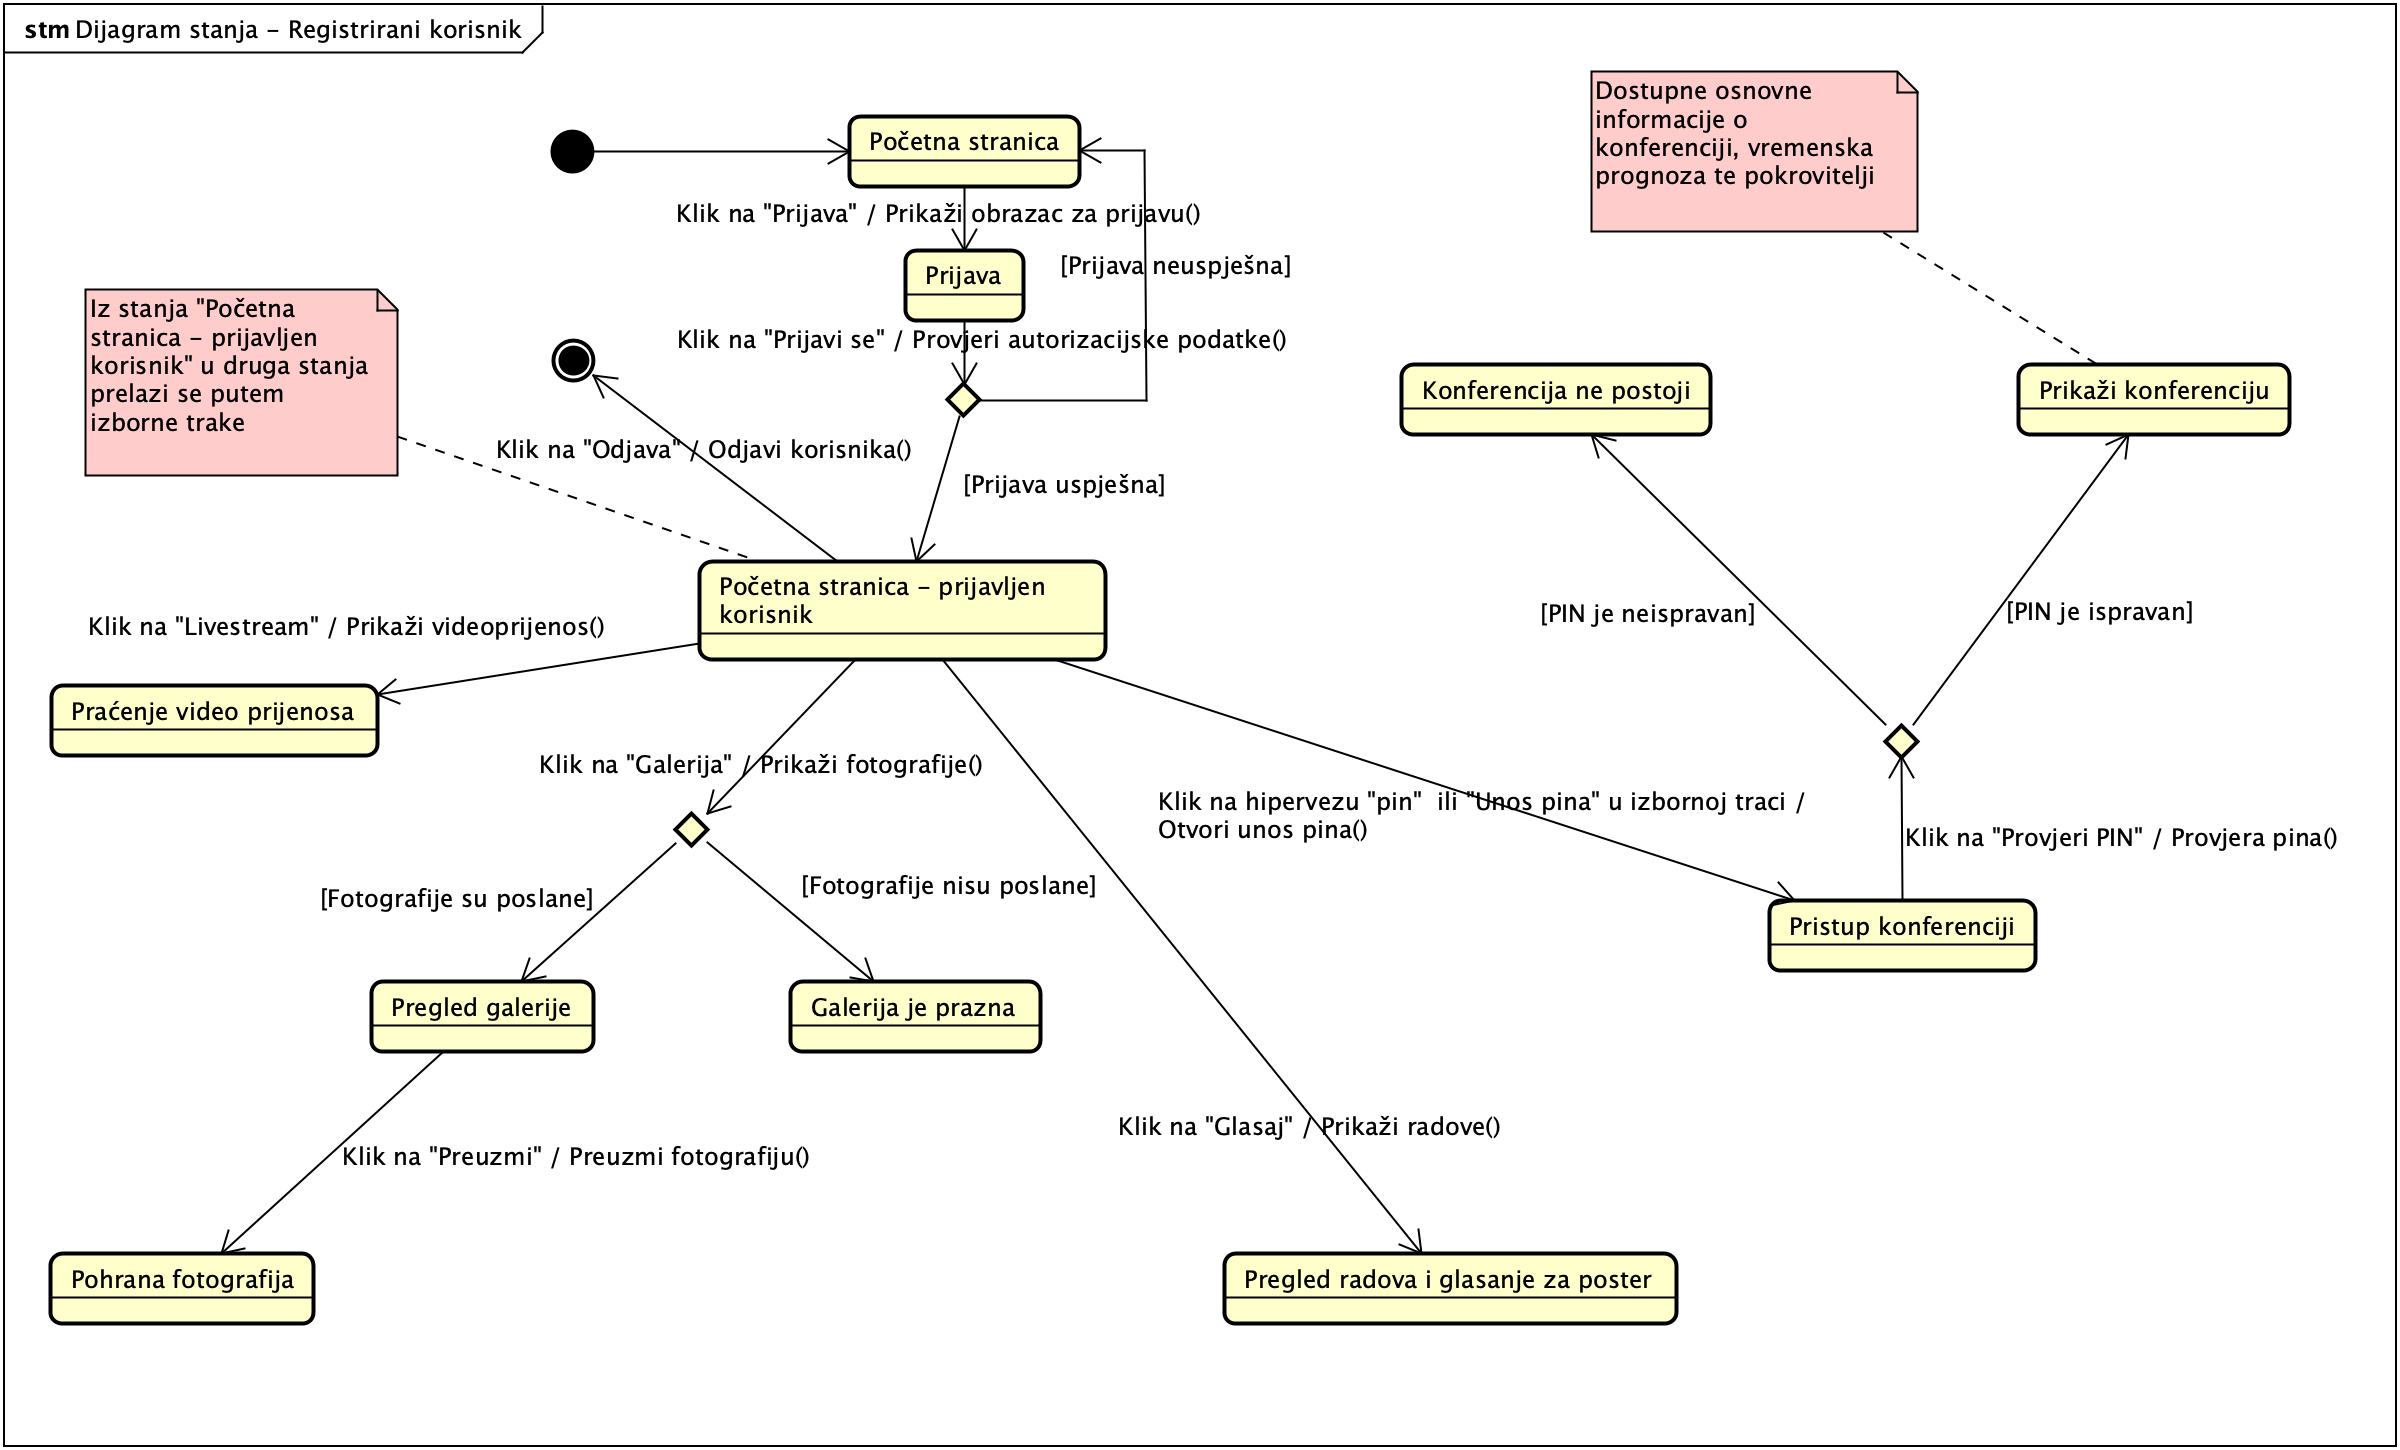
\includegraphics[scale=0.4]{dijagrami/dijagram_stanja.png} %veličina slike u odnosu na originalnu datoteku i pozicija slike
				\centering
				\caption{Dijagram stanja}
				\label{fig:promjene1}
			\end{figure}			
			
			
			\eject 
		
		\section{Dijagram aktivnosti}
			
			Dijagram aktivnosti primjenjuje se za opis modela toka upravljanja ili toka podataka. Ne upotrebljava se za modeliranje događajima poticanog ponašanja. U modeliranju toka upravljanja svaki novi korak poduzima se nakon završenog prethodnog, a naglasak je na jednostavnosti. Na dijagramu 4.8 prikazan je proces glasanja za najbolji rad. Registrirani korisnik se prijavljuje u sustav, a nakon uspješne prijave ima mogućnost prijaviti se na konferenciju. Korisnik se prijavljuje na konferenciju unosom pina te na web aplikaciji vidi mogućnosti povezane s tom konferencijom, uključujući i glasanje za najbolji rad. Odabire koji rad mu je najbolji te glasa za njega. 
			
			\begin{figure}[H]
				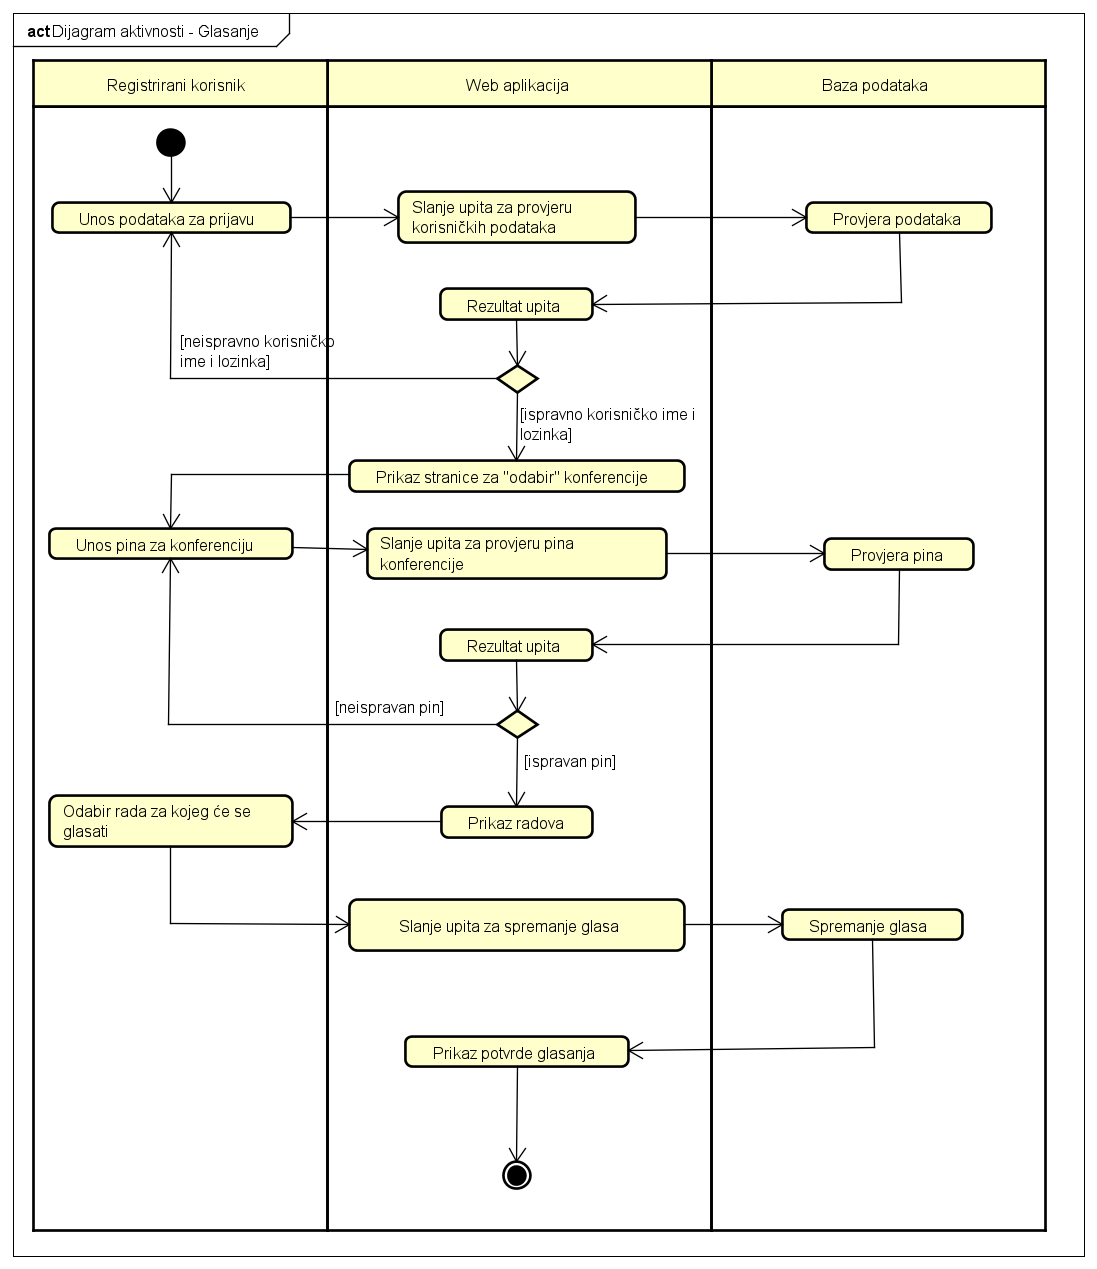
\includegraphics[scale=0.4]{dijagrami/dijagram_aktivnosti.png}%veličina slike u odnosu na originalnu datoteku i pozicija slike
			 	\centering
			 	\caption{Dijagram aktivnosti}
			 	\label{fig:promjene8.1}
			 \end{figure}
			 
			
			\eject
		\section{Dijagram komponenti}
		
			 Dijagram komponenti prikazan na slici opisuje strukturu web aplikacije razdijeljenu na višestruke komponente koje omogućavaju njen rad i interakciju s korisnicima. Pristup sustavu ostvaruje se putem dva osnovna sučelja.
			 
			 Prvo sučelje omogućava dohvat HTML, CSS i JS datoteka koje čine frontend dio aplikacije. Komponente frontenda koriste React biblioteku za izgradnju korisničkog sučelja i organizirane su u logičke cjeline prema tipovima korisnika koji im pristupaju, kao što su superadministratori, administratori, registrirani i neregistrirani korisnici.
			 
			 Router je ključna komponenta koja određuje koja će se datoteka poslužiti temeljem URL-a na koji korisnik dođe. Kroz ovu komponentu, zahtjevi korisnika se usmjeravaju prema odgovarajućim dijelovima aplikacije.
			 
			 Backend dio aplikacije pristupa se preko sučelja koje poslužuje JSON podatke. Ova komponenta se bavi obradom zahtjeva i komunikacijom s bazom podataka. Komunikacija s bazom podataka se odvija preko posebnog SQL API sučelja, a podaci se poslužuju kroz REST API.
			 
			 Svi dijelovi sustava su međusobno povezani i ovise o funkcionalnostima koje pružaju jedni drugima. Na primjer, REST API poslužuje kao most između frontenda i baze podataka, omogućavajući dinamičan i responzivan korisnički doživljaj. Dijagram detaljno prikazuje kako korisnički zahtjevi prolaze kroz različite slojeve aplikacije kako bi se dobili potrebni podaci ili izvršile akcije.
			 
			 \begin{figure}[H]
			 	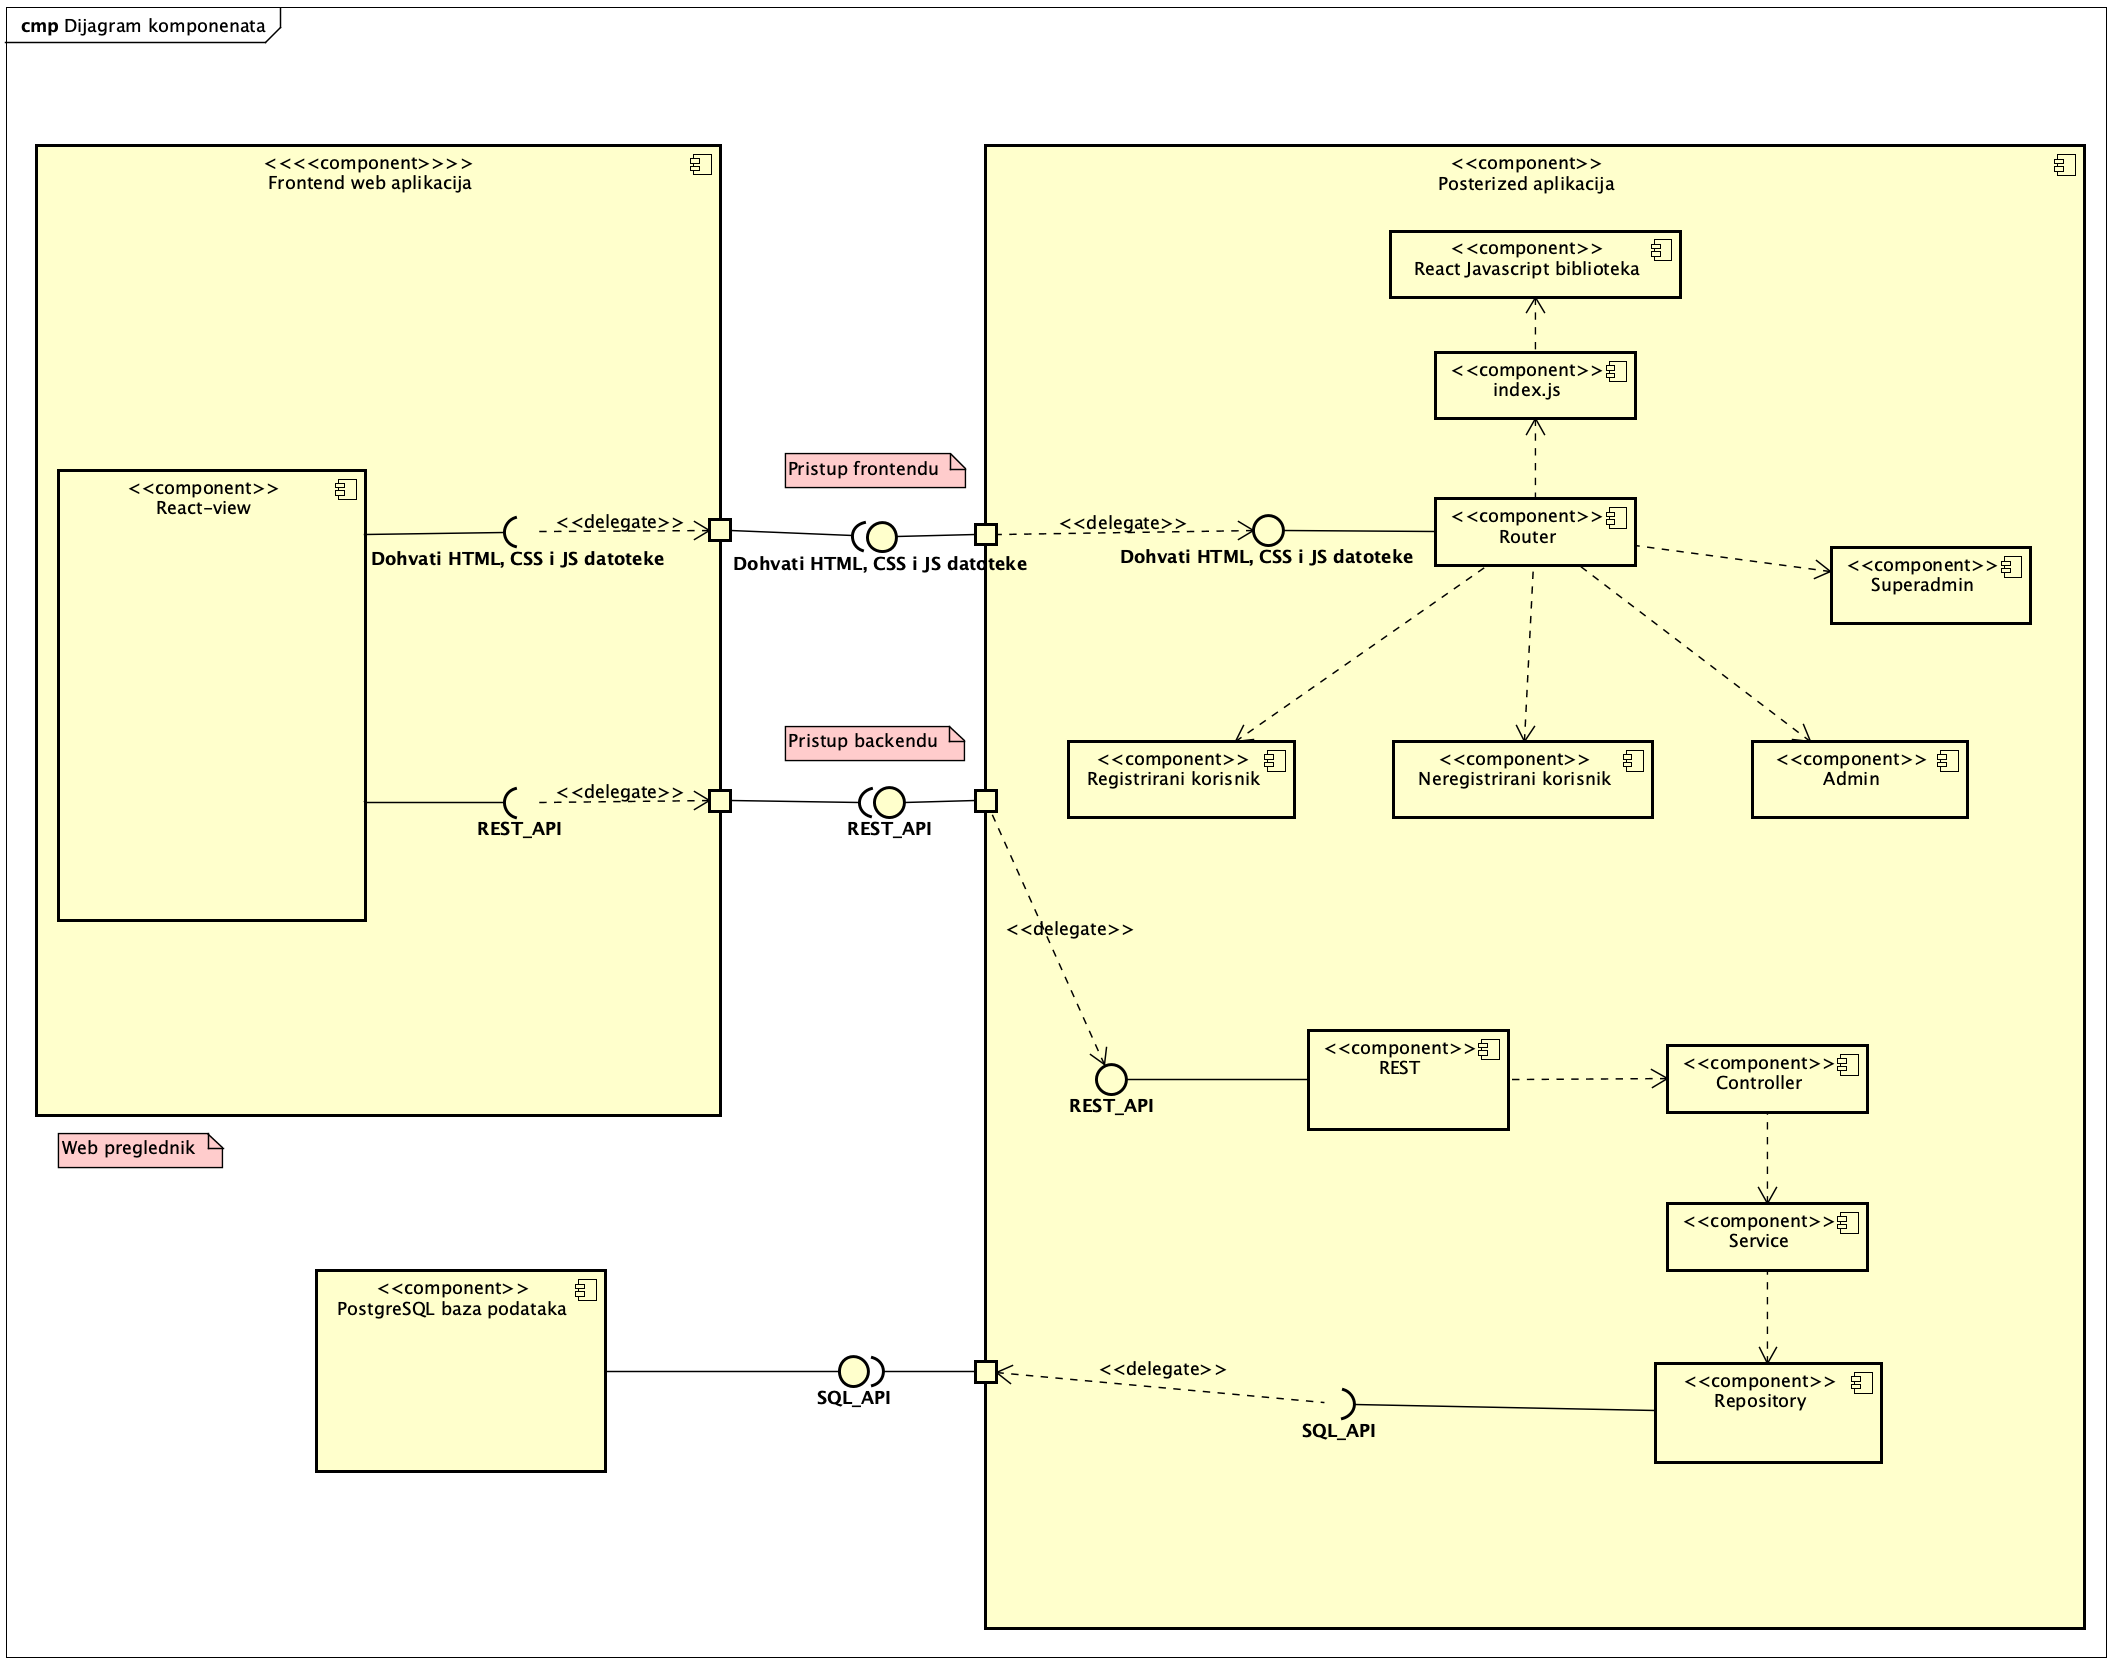
\includegraphics[scale=0.45]{dijagrami/dijagram_komponenata.png}%veličina slike u odnosu na originalnu datoteku i pozicija slike
			 	\centering
			 	\caption{Dijagram komponenata}
			 	\label{fig:promjene}
			 \end{figure}
		